\chapter{Guía Básica de Implementación kernel Linux OpenRISC} \label{app:apendice4}

\section{Descarga del código fuente del proyecto}

Inicialmente se deben descargar los fuentes de la sistema operativo desde el repositorio Git mediante:


\begin{lstlisting}[breaklines]
 usuario@usuario-desktop:~/\$ git clone git://git.openrisc.net/jonas/linux
\end{lstlisting}

Luego de descomprimir el paquete descargado se tendra:

\begin{figure}[h!]
 	\begin{center}
  	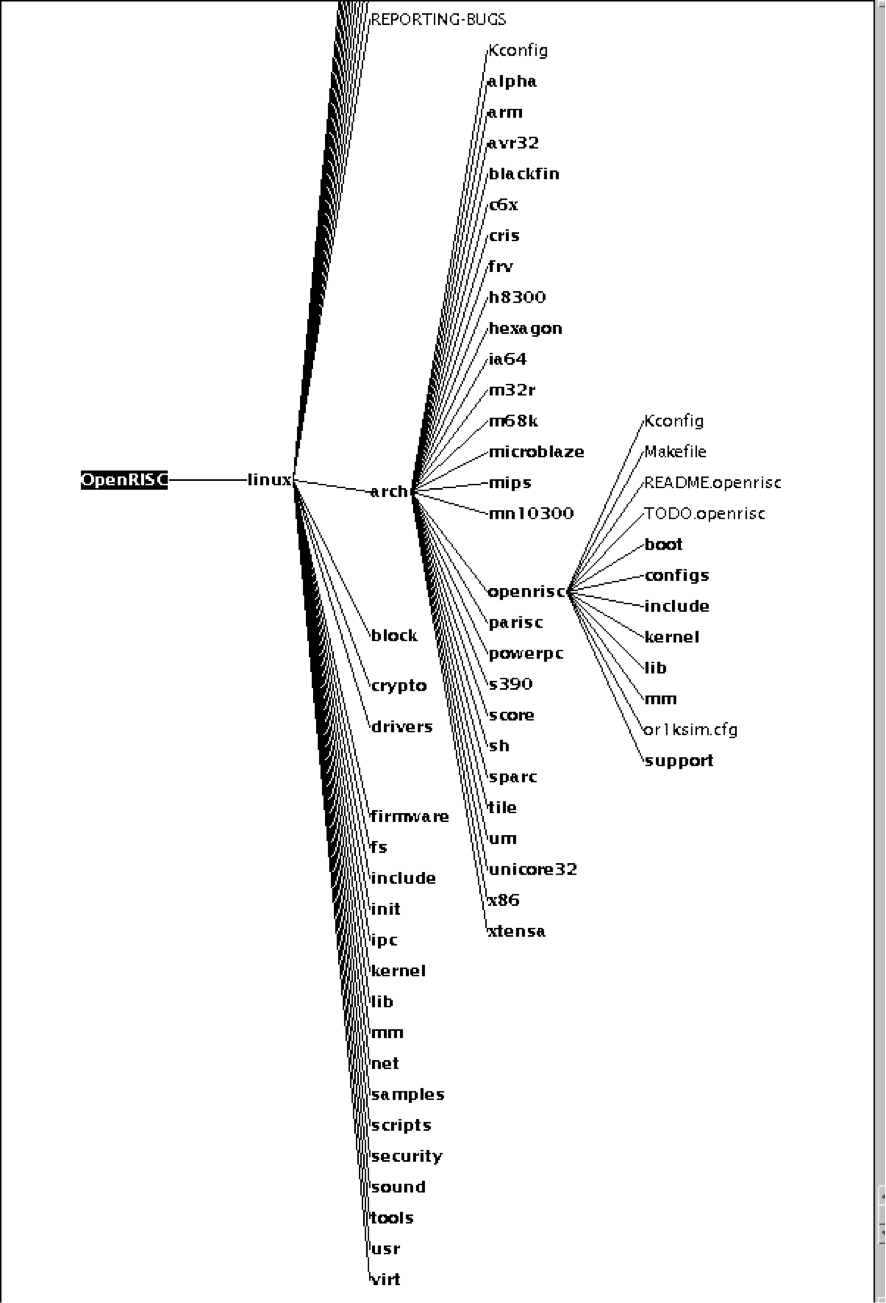
\includegraphics[width=0.5\textwidth,keepaspectratio=true]{./images/kernel}
  	\caption{Arquitectura del OR1200}
  	\label{fig:ArqOR1200}
 	\end{center}
	\end{figure}

\section{Configuración de variables de entorno}

Debe establecer la variable entorno CROSS\_COMPILE en el shell antes de iniciar la construcción del kernel Linux. Debe agregarse la siguiente línea al archivo .bashrc.

\begin{lstlisting}[breaklines]
export CROSS \_COMPILE=or32-elf-
\end{lstlisting}

Es necesario que se reconfiguren las variables mediante:
\begin{lstlisting}[breaklines]
 usuario@usuario-desktop:~/$ source ~/.bashrc
\end{lstlisting}
%%%%%%%%%%%%%%%%%
\section{Construcción del sistema configuración básica}

Tenga en cuenta que hay un binario pre-configurado de BusyBox. Ejecute los siguientes comandos para construir el kernel:


\begin{lstlisting}[breaklines]
usuario@usuario-desktop:~/<directorio de linux>/$ defconfig
usuario@usuario-desktop:~/<directorio de linux>/$ make
\end{lstlisting}

El archivo vmlinux ELF se convierte y se copia en el archivo vmlinux.bin al finalizar el make

\section{Ejecución del kernel en el simulador}

Utilice el siguiente comando para ejecutar el kernel de Linux en el simulador de la arquitectura OpenRISC (or1ksim): 

\begin{lstlisting}[breaklines]
usuario@usuario-desktop:~/<directorio de linux>/$or32-elf-sim -f arch/openrisc/or1ksim.cfg vmlinux
\end{lstlisting}
 
\subsection{Cambio de la configuración del UART}

La primera vez que ejecute el simulador se tiene que cambiar la configuración del UART en el archivo or1ksim  config. Agregar un terminal xterm para utilizar como dispositivo de entrada/salida.

\begin{figure}[h!]
 	\begin{center}
  	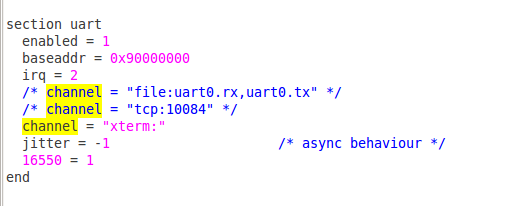
\includegraphics[width=0.5\textwidth,keepaspectratio=true]{./images/uart}
  	\caption{Solución de problema del UART}
  	%\label{fig:ArqOR1200}
 	\end{center}
	\end{figure}


